\documentclass[12pt,a4paper]{scrartcl}
\usepackage[utf8]{inputenc}
\usepackage[english,russian]{babel}
\usepackage{indentfirst}
\usepackage{misccorr}
\usepackage{graphicx}
\usepackage{amsmath}
\usepackage{multirow}
\usepackage{pgfplots}
\usepackage{parskip}
\usepackage[top=1cm, bottom=1cm, left=1cm, right=1cm]{geometry}
\pgfplotsset{compat=1.9}

\begin{document}
	\graphicspath{{py/}}
	
	\newcommand{\ms}{\mathstrut}
	\newcommand{\msp}{\hspace{0.5cm}}
	\newcommand{\al}{\alpha}
	\newcommand{\dg}{^\circ}
	\newcommand{\dif}{\mathrm{d}}
	\newcommand{\qd}[2]{^{\frac{#1}{#2}}}
	\newcommand{\qdm}[2]{^{-\frac{#1}{#2}}}
	\newcommand{\lm}[2]{\underset{#1 \rightarrow #2}{\lim}}
	\newcommand{\sfrac}[2]{\dfrac{\strut #1}{\strut #2}}
	\newcommand{\equal}[1]{\overset{(#1)}{=}}
	\newcommand{\linevdots}{\ \raisebox{-.08\height}{\vdots}\ }
	\newcommand{\linecvdots}{\ \raisebox{-.08\height}{\vdots}\hspace{-0.13cm}\raisebox{.15\height}{\cancel{\phantom{a}}\hspace{0.06cm}}}
	\newcommand{\combox}[1]{\ms \msp \msp \begin{minipage}{0.95\linewidth}
			#1
	\end{minipage}}
	
	\newtheorem{pr}{Задача}
	\newtheorem{ex}{Пример}
	\newtheorem{dfn}{Def}
	\newtheorem{theorem}{Th}
	
	\newenvironment{slv}{\ms \msp \textit{Решение:}}{}
	\newenvironment{proof}{\ms \msp \textit{Доказательство: }}{\hfill $\square$}
	
	\begin{titlepage}
		
		\vspace*{\fill}
		
		\begin{center}
			
\includegraphics[scale=0.8]{MIPT.png}
			\\[0.7cm]\Huge Московский Физико-Технический Институт\\(национальный исследовательский университет)
			\\[2cm]\LARGE Отчет по эксперименту
			\\[0.5cm]\noindent\rule{\textwidth}{1pt}
			\\\Huge\textbf{Скин-эффект в полом цилиндре}
			\\[-0.5cm]\noindent\rule{\textwidth}{1pt}
		\end{center}
		
		\begin{flushleft}
			\textit{Работа №3.7.1; дата: 30.09.22}\hfill\textit{Семестр: 3}
		\end{flushleft}
		
		\vspace*{\fill}
		
		\begin{flushleft}
			Выполнил: \hspace{\fill} Группа:
			\\Кошелев Александр \hspace{\fill} Б05-105
		\end{flushleft}
	\end{titlepage}
	
	%Страница 2
	
	\begin{flushleft}
		\footnotesize{Скин-эффект в полом цилиндре} \hspace{\fill} \footnotesize{2}
		\\[-0.3cm]\noindent\rule{\textwidth}{0.3pt}
	\end{flushleft}
	
	\section{Аннотация}
	
	\textbf{Цель работы: }
	
	Исследование проникновения переменного магнитного поля в медный полый цилиндр.
		
	\textbf{Экспериментальная установка:}
		
	\begin{center}
		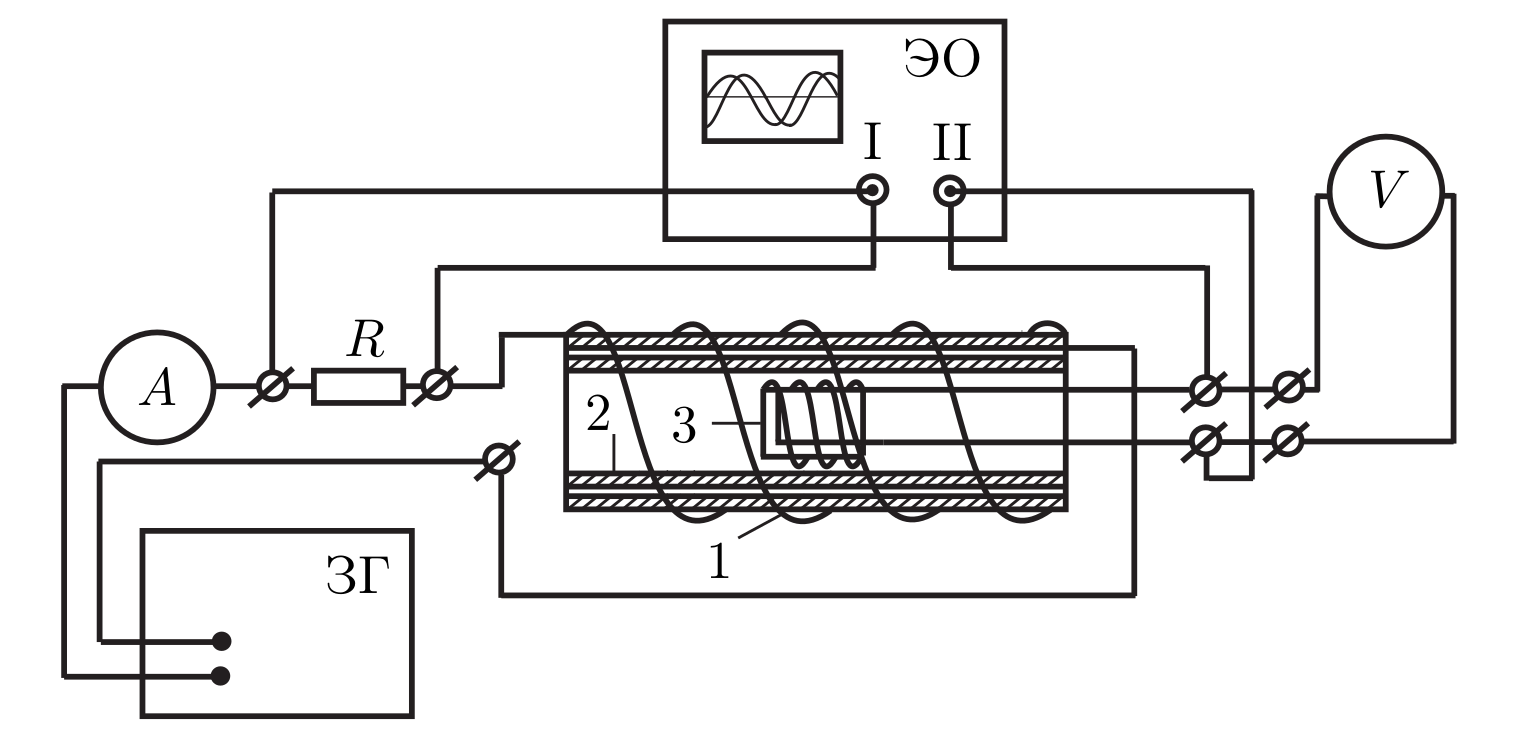
\includegraphics[scale=0.25]{PIC_1.png}
		\\\textbf{Рис. 1:} Экспериментальная установка
	\end{center}	

	Переменное магнитное поле создаётся с помощью соленоида, намотанного на полый цилиндрический каркас 1 из поливинилхлорида, который подключается к генератору звуковой частоты. Внутри соленоида расположен медный цилиндрический экран 2. Для измерения магнитного поля внутри экрана используется измерительная катушка 3.
	Необходимые параметры соленоида, экрана и измерительной катушки указаны на установке. Действующее значение переменного тока в цепи соленоида измеряется амперметром $A$, а действующее значение напряже	ния на измерительной катушке измеряет вольтметр $V$. Для измерения сдвига фаз между током в цепи соленоида и напряжением на измерительной катушке используется двухканальный осциллограф. На вход одного
	канала подаётся напряжение с резистора $R$, которое пропорционально току, а на вход второго канала — напряжение с измерительной катушки.
		
	\textbf{В работе используются:}
	
	Генератор звуковой частоты, соленоид, намотанный на полый цилиндрический каркас из диэлектрика, медный экран в виде трубки, измерительная катушка,	амперметр, вольтметр, осциллограф.
	
	\section{Теоретические сведения}
	
	В работе изучается скин-эффект в длинном тонкостенном медном цилиндре, помещённом внутрь соленоида.
	
	Пусть цилиндр достаточно длинный, так что в нём можно пренебречь краевыми эффектами. В этом приближении магнитное поле $\vec{H}$ всюду направлено по оси системы (ось $z$), а вихревое электрическое поле $\vec{E}$ будет всюду перпендикулярно радиусу, то есть линии поля образуют соосные окружности. 
	
	
	\newpage
	
	%Страница 3
	
	\begin{flushleft}
		\footnotesize{Скин-эффект в полом цилиндре} \hspace{\fill} \footnotesize{3}
		\\[-0.3cm]\noindent\rule{\textwidth}{0.3pt}
	\end{flushleft}
	
	\begin{center}
		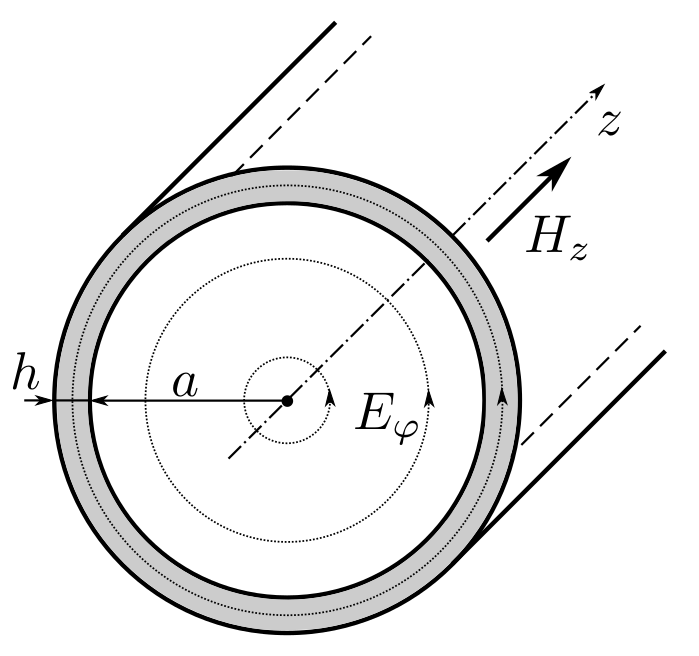
\includegraphics[scale=0.3]{PIC_2.png}
		\\\textbf{Рис. 2:} Электрическое и магнитное поле в тонкостенном цилиндре
	\end{center}
	
	Все	величины будем считать колеблющимися по гармоническому закону с некоторой частотой $\omega$, задаваемой частотой колебания тока в соленоиде. Тогда для ненулевых компонент поля можно записать:
	
	$$H_z = H(r)\exp(i\omega t)\ \ \ \ \ \ \ \ E_\varphi = E(r)\exp(i\omega t)$$
	
	где $H(r)$ и $E(r)$ — комплексные амплитуды колебаний соответствующих полей, зависящие только от расстояния $r$ до оси системы. Заметим, что на границе цилиндра должны быть непрерывны касательные к поверхности компоненты как $E$, так и $B$, поэтому функции $E(r)$ и $H(r)$ непрерывны во всей исследуемой области.
	
	Пусть длинный полый цилиндр имеет радиус $a$ и толщину стенки $h \ll a$. Последнее условие позволяет для описания поля внутри стенки	ограничиться одномерным приближением. При этом для полного решения задачи необходимо вычислить и распределение поля внутри цилиндра.
	
	Поскольку внутри цилиндра ток отсутствует, магнитное поле там является однородным (аналогично полю внутри пустого соленоида): $H_z(r, t) = H_1 \exp(i \omega t)$, где $H_1 = \mathrm{const}$ — амплитуда поля на внутренней поверхности цилиндра. Для нахождения вихревого электрического поля воспользуемся законом электромагнитной индукции в интегральной форме:
	
	$$E_\varphi \cdot 2\pi r = -\mu_0 \pi r^2 \cdot \sfrac{\dif H_z}{\dif t} \implies E(r) = -\sfrac{1}{2} \mu_0 r \cdot i \omega H_1$$
	
	Отсюда получим связь амплитуд колебаний электрического и магнитного полей на внутренней $(r = a)$ границе цилиндра:
	
	$$E_1 = -\sfrac{1}{2} \mu_0 a \cdot i \omega H_1$$
	
	Данное соотношение используем далее как дополнительное граничное условие для задачи о распределении поля внутри стенки.
	
	Поле внутри тонкой стенки цилиндра («экрана») описывается уравнением скин-эффекта (уравнением диффузии поля) в плоской геометрии. Поместим начало отсчёта на внешнюю поверхность цилиндра и направим ось $x$ к оси системы, и запишем дифференциаль ное уравнение для комплексной амплитуды магнитного поля:
	\newpage
	
	%Страница 4
	
	\begin{flushleft}
	\footnotesize{Скин-эффект в полом цилиндре} \hspace{\fill} \footnotesize{4}
	\\[-0.3cm]\noindent\rule{\textwidth}{0.3pt}
\end{flushleft}
	
	\begin{center}
		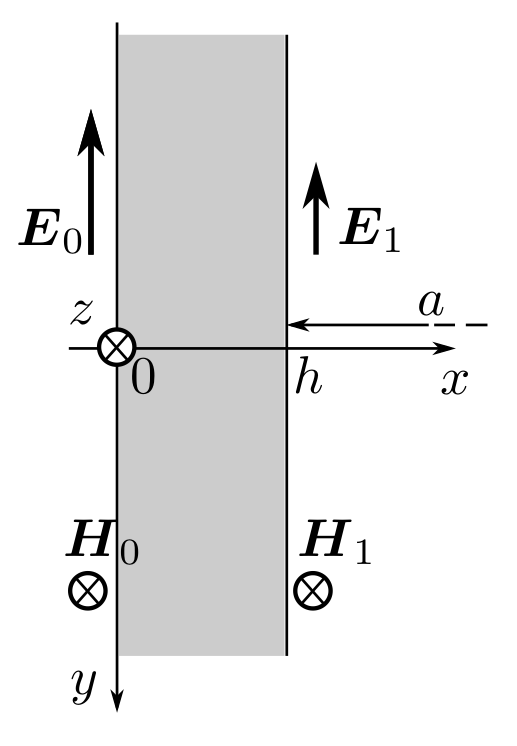
\includegraphics[scale=0.25]{PIC_3.png}
		\\\textbf{Рис. 3:} Поле внутри стенки цилиндра
	\end{center}
	
	$$\sfrac{\dif^2 H}{\dif x^2} = i \omega \sigma \mu_0 H$$
	
	(Для медного цилиндра можно положить $\mu \approx 1$). Граничные условия зададим в виде:
	
	$$H(0) = H_0 \ \ \ \ \ \ \ \ H(h) = H_1$$
	
	
	Здесь $H_0$ -- амплитуда колебаний магнитного поля на внешней границе цилиндра. Её значение определяется только током в обмотке соленоида, и совпадает с полем внутри соленоида в отсутствие цилиндра. Величина $H_1$ также поддаётся непосредственному измерению -- это амплитуда колебаний однородного поля внутри цилиндра. Поля $H_0$ и $H_1$ не являются независимыми -- они связаны через решение уравнений поля вне проводника, т. е. внутри «экрана».
	
	Решение ищем в виде:
	
	$$H(x) = A\exp(\alpha x) + B\exp(-\alpha x)$$
	
	где $A, B$ — определяемые из граничных условий константы,
	
	$$\alpha = \sqrt{i \omega \sigma \mu_0} = \sfrac{1 + i}{\delta} = \sfrac{\sqrt{2}}{\delta}\exp(i\pi / 4)$$
	
	Из предыдущих уравнений $A + B = H_0$, поэтому можно записать:
	
	$$H(x) = H_0\exp(-\alpha x) + 2B\sinh (\alpha x)$$
	
	Выразим электрическое поле из закона Ампера (7.21). В одномерном случае:
	
	$$E(x) = \sfrac{1}{h} \cdot \sfrac{\dif H}{\dif x} = \sfrac{\alpha}{\sigma}(-H_0\exp(-\alpha x) + 2B \cosh(\alpha x))$$
	
	
	\newpage
	%Страница 5
	
	\begin{flushleft}
		\footnotesize{Скин-эффект в полом цилиндре} \hspace{\fill} \footnotesize{5}
		\\[-0.3cm]\noindent\rule{\textwidth}{0.3pt}
	\end{flushleft}
	
	Далее положим $x = h$, воспользуемся условиями, и, исключив константу $B$, получим после преобразований связь между $H_0$ и $H_1$:
	
	$$H_1 = \sfrac{H_0}{\cosh(\alpha h) + \frac{1}{2}\alpha a \sinh(\alpha h)}$$
	
	Рассмотрим предельные случаи:
	
	1.При малых частотах толщина скин-слоя превосходит толщину цилиндра $\delta \gg h$. Тогда $|\alpha h| \ll 1$, поэтому $\cosh \alpha h \approx 1$, $\sinh \alpha x \approx \alpha x$ и
	
	$$H_1 \approx \sfrac{H_0}{1 + i\frac{ah}{\delta^2}}$$
	
	Заметим, что величина $ah / \delta^2$ в общем случае не мала, поскольку при	$h \ll a$ возможна ситуация $h \ll \delta \ll a$. Отношение модулей амплитуд здесь будет равно
	
	$$\sfrac{|H_1|}{|H_0|} = \sfrac{1}{\sqrt{1 + \frac{1}{4} (ah\sigma \mu_0 \omega)^2}}$$
	
	При этом колебания $H_1$ отстают по фазе от $H_0$ на угол $\psi$, определяемый равенством $\tan \psi = ah / \delta^2$.
	
	2. При достаточно больших частотах толщина скин-слоя станет меньше толщины стенки: $\delta \ll h$. Тогда $\alpha h \gg 1$ и $\alpha a \gg 1$, а также $\sinh \alpha h \approx \cosh \alpha h \approx \frac{1}{2} \exp{\alpha h}$. Выражение (6) с учётом (5) переходит в
	
	$$\sfrac{H_1}{H_0} = \sfrac{2\sqrt{2}\delta}{a} \exp\left(-\frac{h}{\delta} - i\left(\sfrac{\pi}{4} - \sfrac{h}{\delta}\right)\right)$$
	
	\begin{center}
		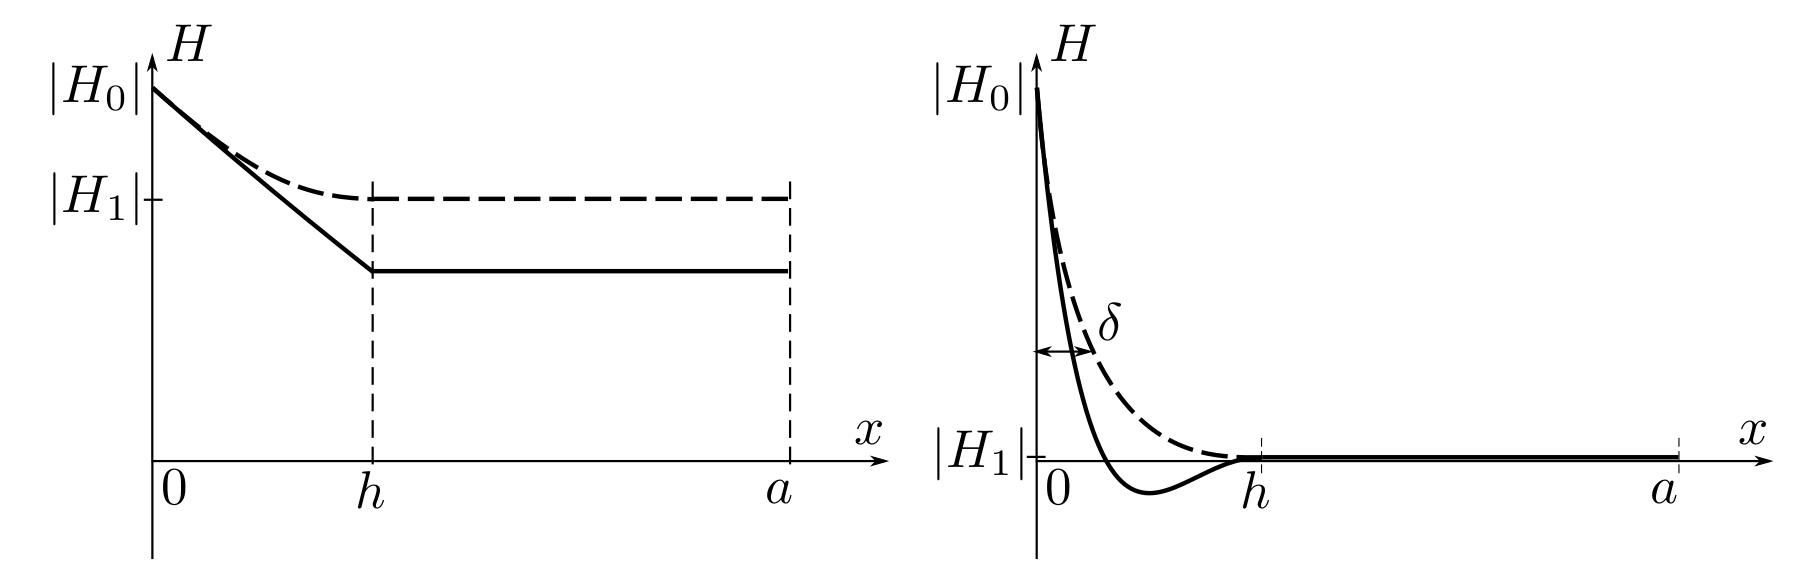
\includegraphics[scale=0.25]{PIC_4.png}
		\\\textbf{Рис. 4:} Распределение амплитуды колебаний магнитного поля (пунктир) и его мгновенного значения при некотором $t$ (сплошная) в зависимости от расстояния до внешней стенки цилиндра. Слева случай низких частот $\delta \gg h$, справа	-- скин-эффект при высоких частотах $\delta \ll h$
	\end{center}

	Как видно из предыдущей формулы, в этом пределе поле внутри цилиндра по модулю в $\frac{2\sqrt{2}\delta}{a\exp(-h/\delta)}$ раз меньше, чем снаружи, и, кроме того, запаздывает
	по фазе на
	
	$$\psi = \sfrac{\pi}{4} + h\sqrt{\sfrac{\omega \sigma \mu_0}{2}}$$
	
	На Рис. 4 схематично изображено распределение магнитного поля от координаты в двух рассмотренных предельных случаях.
	
	
	\newpage
	%Страница 6
	
	\begin{flushleft}
		\footnotesize{Скин-эффект в полом цилиндре} \hspace{\fill} \footnotesize{6}
		\\[-0.3cm]\noindent\rule{\textwidth}{0.3pt}
	\end{flushleft}
	
	\section{Проведение эксперимента}
	
	\paragraph{Исследование области низких частот} \hfill
	
	Рассчитаем частоту, при которой толщина стенок экрана равна скиновой длине и получим $\nu_h = \frac{1}{\pi \sigma \mu \mu_0 h^2} \approx 2250$ Hz.
	
	Проведем измерения и рассчитаем $\xi$:
	
	\begin{center}
		\begin{tabular}{|c|c|c|c|}
			\hline
			$\nu$, Hz & $U$, mV & $I$, mA & $\xi \cdot 10^{-5}$, V/(Hz$\cdot$mA)
			\\\hline
			112 & 30.0 & 20.09 & 1.33 $\pm$ 0.13
			\\\hline
			184 & 37.4 & 18.90 & 1.08 $\pm$ 0.08
			\\\hline
			256 & 40.7 & 18.17 & 0.88 $\pm$ 0.07
			\\\hline
			328 & 42.2 & 17.72 & 0.73 $\pm$ 0.05
			\\\hline
			400 & 42.9 & 17.40 & 0.62 $\pm$ 0.04
			\\\hline
			472 & 43.2 & 17.16 & 0.53 $\pm$ 0.04
			\\\hline
			544 & 43.3 & 16.95 & 0.47 $\pm$ 0.03
			\\\hline
			616 & 43.1 & 16.75 & 0.42 $\pm$ 0.03
			\\\hline
			688 & 43.0 & 16.56 & 0.37 $\pm$ 0.02
			\\\hline
			760 & 42.7 & 16.39 & 0.34 $\pm$ 0.02
			\\\hline
			832 & 42.4 & 16.19 & 0.32 $\pm$ 0.02
			\\\hline
		\end{tabular}
		\\\textbf{Табл. 1:} Определение $\xi = U/\nu I$ в области низких частот
	\end{center}

	Сделаем дополнительную таблицу для построения графика:

	\begin{center}
		\begin{tabular}{|c|c|}
			\hline
			$\nu^2 \cdot 10^{-5}$, Hz$^2$ & $1/\xi^2 \cdot 10^{10}$, (Hz$\cdot$mA/V)$^2$
			\\\hline
			0.13 $\pm$ 0.002 & 0.57 $\pm$ 0.058
			\\\hline
			0.34 $\pm$ 0.007 & 0.87 $\pm$ 0.070
			\\\hline
			0.66 $\pm$ 0.013 & 1.31 $\pm$ 0.098
			\\\hline
			1.08 $\pm$ 0.022 & 1.90 $\pm$ 0.138
			\\\hline
			1.60 $\pm$ 0.032 & 2.64 $\pm$ 0.189
			\\\hline
			2.23 $\pm$ 0.045 & 3.52 $\pm$ 0.250
			\\\hline
			2.96 $\pm$ 0.059 & 4.54 $\pm$ 0.322
			\\\hline
			3.79 $\pm$ 0.076 & 5.73 $\pm$ 0.409
			\\\hline
			4.73 $\pm$ 0.095 & 7.02 $\pm$ 0.503
			\\\hline
			5.78 $\pm$ 0.116 & 8.50 $\pm$ 0.613
			\\\hline
			6.92 $\pm$ 0.138 & 10.09 $\pm$ 0.733
			\\\hline
		\end{tabular}
		\\\textbf{Табл. 2:} График зависимости $(1/\xi^2)(\nu^2)$ в области низких частот
	\end{center}
	
	Из теории зависимость имеет вид:
	
	$$\sfrac{1}{\xi^2} = \sfrac{1}{\xi_0^2} + \sfrac{(ah\sigma \mu_0 \pi)^2}{\xi_0^2}\nu^2$$
	
	\newpage
	%Страница 7
	
	\begin{flushleft}
		\footnotesize{Скин-эффект в полом цилиндре} \hspace{\fill} \footnotesize{7}
		\\[-0.3cm]\noindent\rule{\textwidth}{0.3pt}
	\end{flushleft}
	
	\begin{center}
		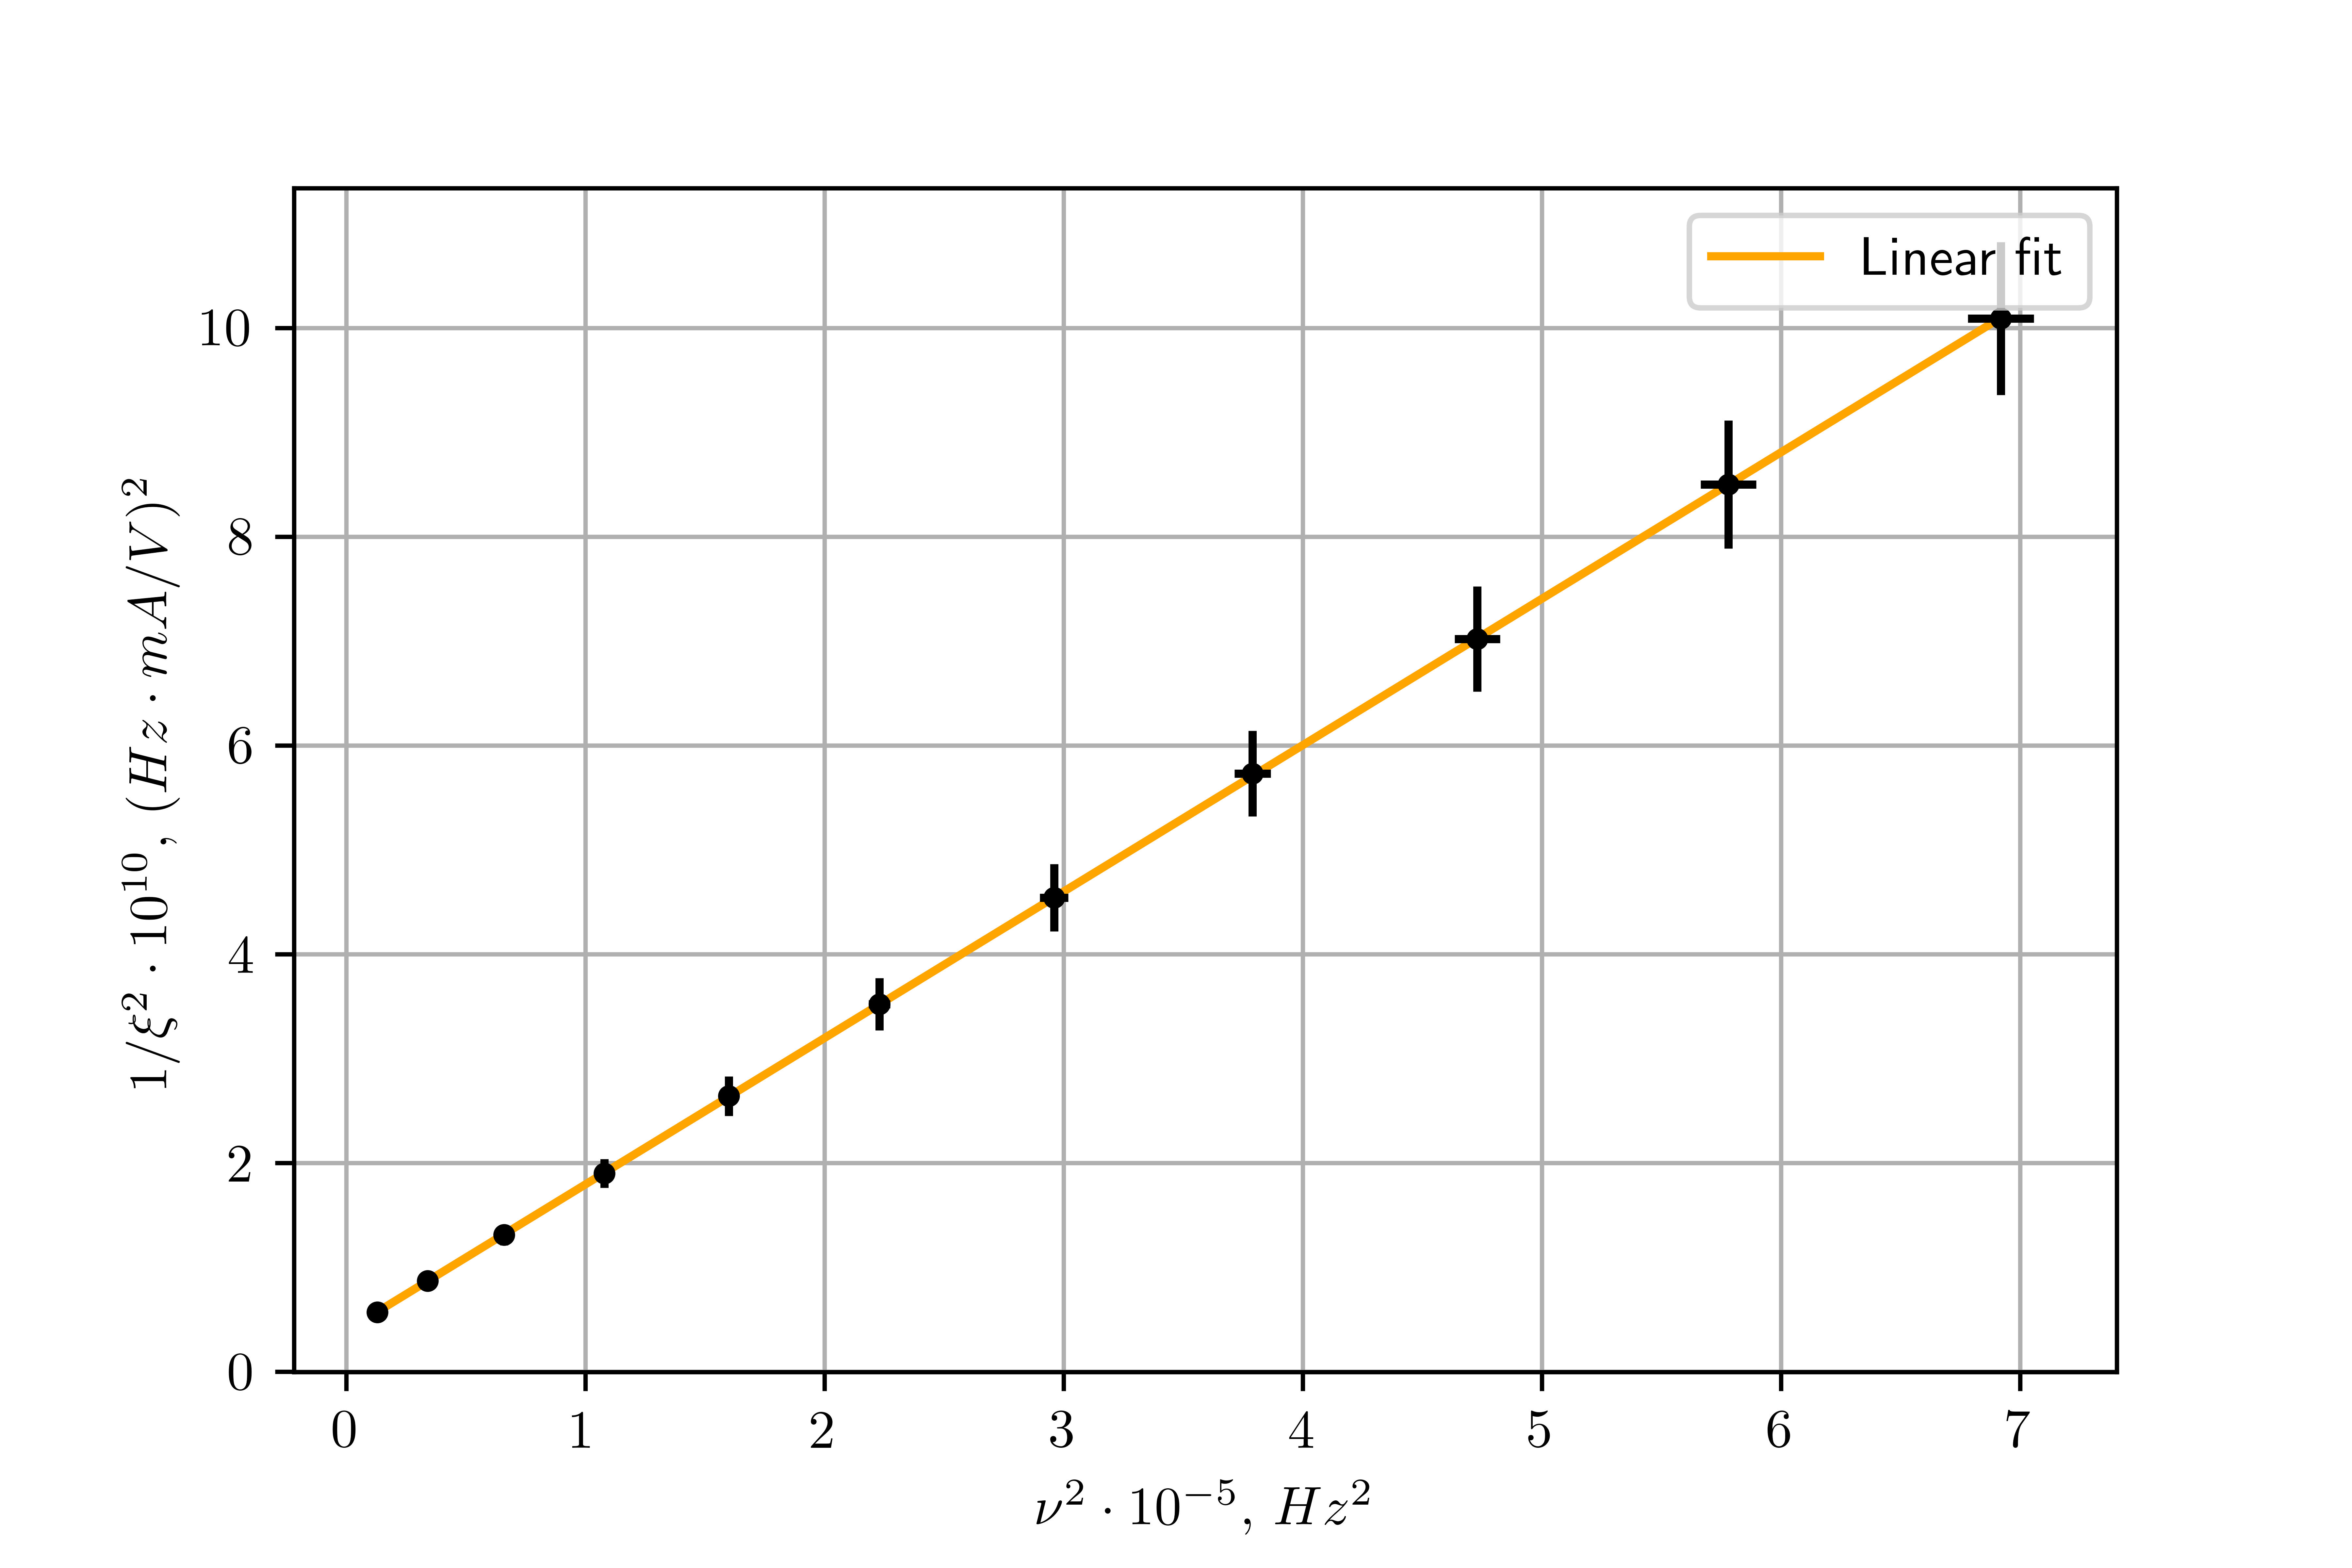
\includegraphics[scale=1]{PIC_5.png}
		\\\textbf{Рис. 5:} График зависимости $(1/\xi^2)(\nu^2)$ в области низких частот
	\end{center}
	
	Точки хорошо ложатся на прямую, положив вид зависимости $1/\xi^2 = k\nu^2 + b$, методом линейной аппроксимации получаем:
	
	$$k = (14030 \pm 10)\, \left(\sfrac{\text{A}}{\text{V}}\right)^2 \ \ \ \ \ \ \ \ b = (3910 \pm 40) \left(\sfrac{\text{Hz} \cdot \text{A}}{\text{V}}\right)^2$$
	
	Потому:
	
	$$\xi_0 = (1.6 \pm 0.03) \cdot 10^{-2} \left(\sfrac{\text{Ohm}}{\text{Hz}}\right)^2 \ \ \ \ \ \ \ \ \sigma = (4.5 \pm 0.1) \cdot 10^7\,\sfrac{\text{S}}{\text{m}}$$
	
	
	\paragraph{Исследование области высоких частот} \hfill
	
	\begin{center}
		\begin{tabular}{|c|c|c|}
			\hline
			$\nu$, kHz & $\nu^{1/2}$, Hz$^{1/2}$ & $\Delta \psi$
			\\\hline
			2.5 $\pm$ 0.1 & 50 $\pm$ 10 & 0.32 $\pm$ 0.01
			\\\hline
			5.0 $\pm$ 0.1 & 70 $\pm$ 7 & 0.63 $\pm$ 0.01
			\\\hline
			7.5 $\pm$ 0.1 & 86 $\pm$ 6 & 0.99 $\pm$ 0.01
			\\\hline
			10.0 $\pm$ 0.1 & 100 $\pm$ 5 & 1.24 $\pm$ 0.01
			\\\hline
			12.5 $\pm$ 0.1 & 111 $\pm$ 5 & 1.40 $\pm$ 0.01
			\\\hline
			15.0 $\pm$ 0.1 & 122 $\pm$ 4 & 1.41 $\pm$ 0.01
			\\\hline
			17.5 $\pm$ 0.1 & 132 $\pm$ 4 & 1.26 $\pm$ 0.01
			\\\hline
			20.0 $\pm$ 0.1 & 141 $\pm$ 4 & 0.90 $\pm$ 0.01
			\\\hline
			22.5 $\pm$ 0.1 & 150 $\pm$ 3 & 0.73 $\pm$ 0.01
			\\\hline
			25.0 $\pm$ 0.1 & 158 $\pm$ 3 & 0.57 $\pm$ 0.01
			\\\hline
			27.5 $\pm$ 0.1 & 166 $\pm$ 3 & 0.34 $\pm$ 0.01
			\\\hline
		\end{tabular}
		\\\textbf{Табл. 3:} Зависимость $\Delta \psi(\nu^{1/2})$
	\end{center}
	
	
	\newpage
	%Страница 8
	
	\begin{flushleft}
		\footnotesize{Скин-эффект в полом цилиндре} \hspace{\fill} \footnotesize{8}
		\\[-0.3cm]\noindent\rule{\textwidth}{0.3pt}
	\end{flushleft}
	
	\begin{center}
		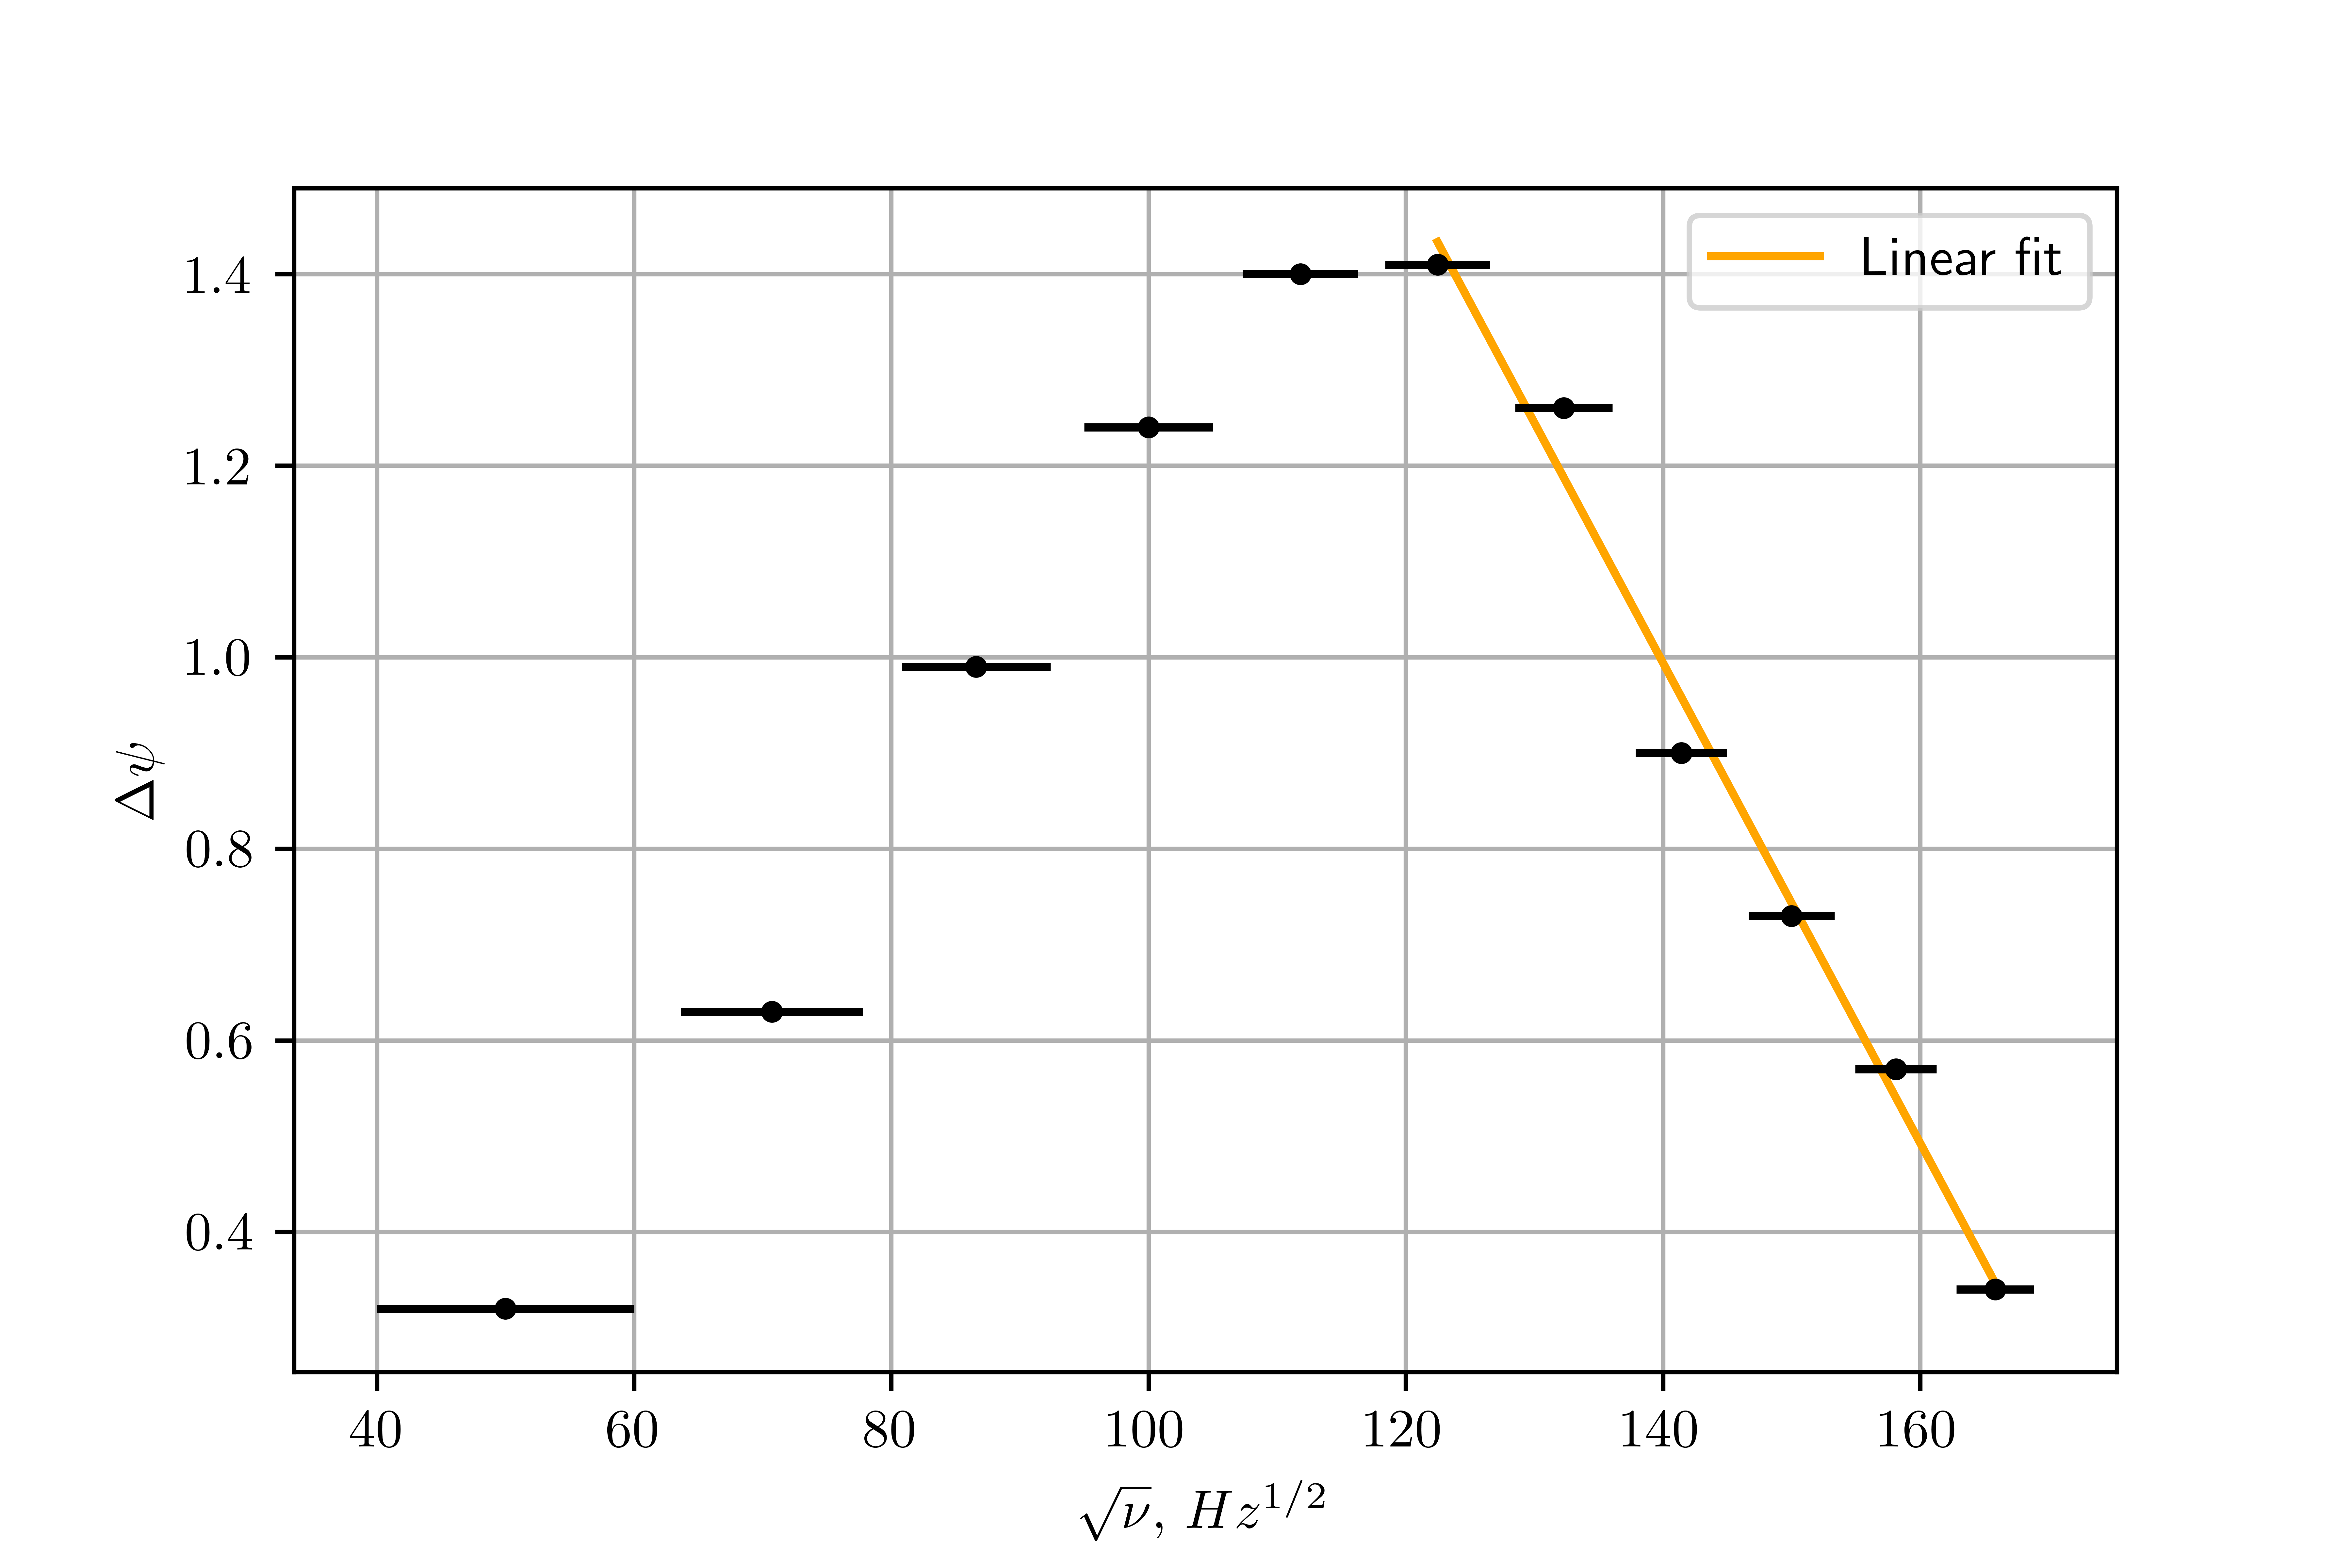
\includegraphics[scale=1]{PIC_6.png}
		\\\textbf{Рис. 6:} График зависимости $\Delta \psi(\nu^{1/2})$
	\end{center}
	
	Точки хорошо ложатся на прямую, положив вид зависимости $\Delta \psi = -k\nu^{1/2} + b$, методом линейной аппроксимации получаем:
	
	$$k = (0.025 \pm 0.001)\,\text{Hz}^{-1/2} \ \ \ \ \ \ \ \ b = (4.5 \pm 0.5)$$
	
	При этом:
	
	$$\sigma = \left(\sfrac{k}{h}\right)^2 \cdot \sfrac{\pi}{\mu_0} = (7.0 \pm 1.2) \cdot 10^7 \sfrac{S}{m}$$
	
	\newpage
	%Страница 9
	
	\begin{flushleft}
		\footnotesize{Скин-эффект в полом цилиндре} \hspace{\fill} \footnotesize{9}
		\\[-0.3cm]\noindent\rule{\textwidth}{0.3pt}
	\end{flushleft}
	
	\paragraph{Общий вид зависимости $(|H_1|/|H_0|)(\nu)$} \hfill
	
	\begin{center}
		\begin{tabular}{|c|c|}
			\hline
			$\nu$, Hz & $|H_1|/|H_0|$
			\\\hline
			112 & 82.93
			\\\hline
			184 & 67.20
			\\\hline
			256 & 54.67
			\\\hline
			328 & 45.37
			\\\hline
			400 & 38.51
			\\\hline
			472 & 33.33
			\\\hline
			544 & 29.34
			\\\hline
			616 & 26.10
			\\\hline
			688 & 23.58
			\\\hline
			760 & 21.44
			\\\hline
			832 & 19.67
			\\\hline
			2500 & 6.58
			\\\hline
			5000 & 3.15
			\\\hline
			7500 & 2.0
			\\\hline
			10000 & 1.44
			\\\hline
			12500 & 0.89
			\\\hline
			15000 & 0.81
			\\\hline
			17500 & 0.80
			\\\hline
			20000 & 0.73
			\\\hline
			22500 & 0.72
			\\\hline
			25000 & 0.75
			\\\hline
			27500 & 0.86
			\\\hline
		\end{tabular}
		\\\textbf{Табл. 4:} Зависимость $(|H_1|/|H_0|)(\nu)$
	\end{center}

	\begin{center}
		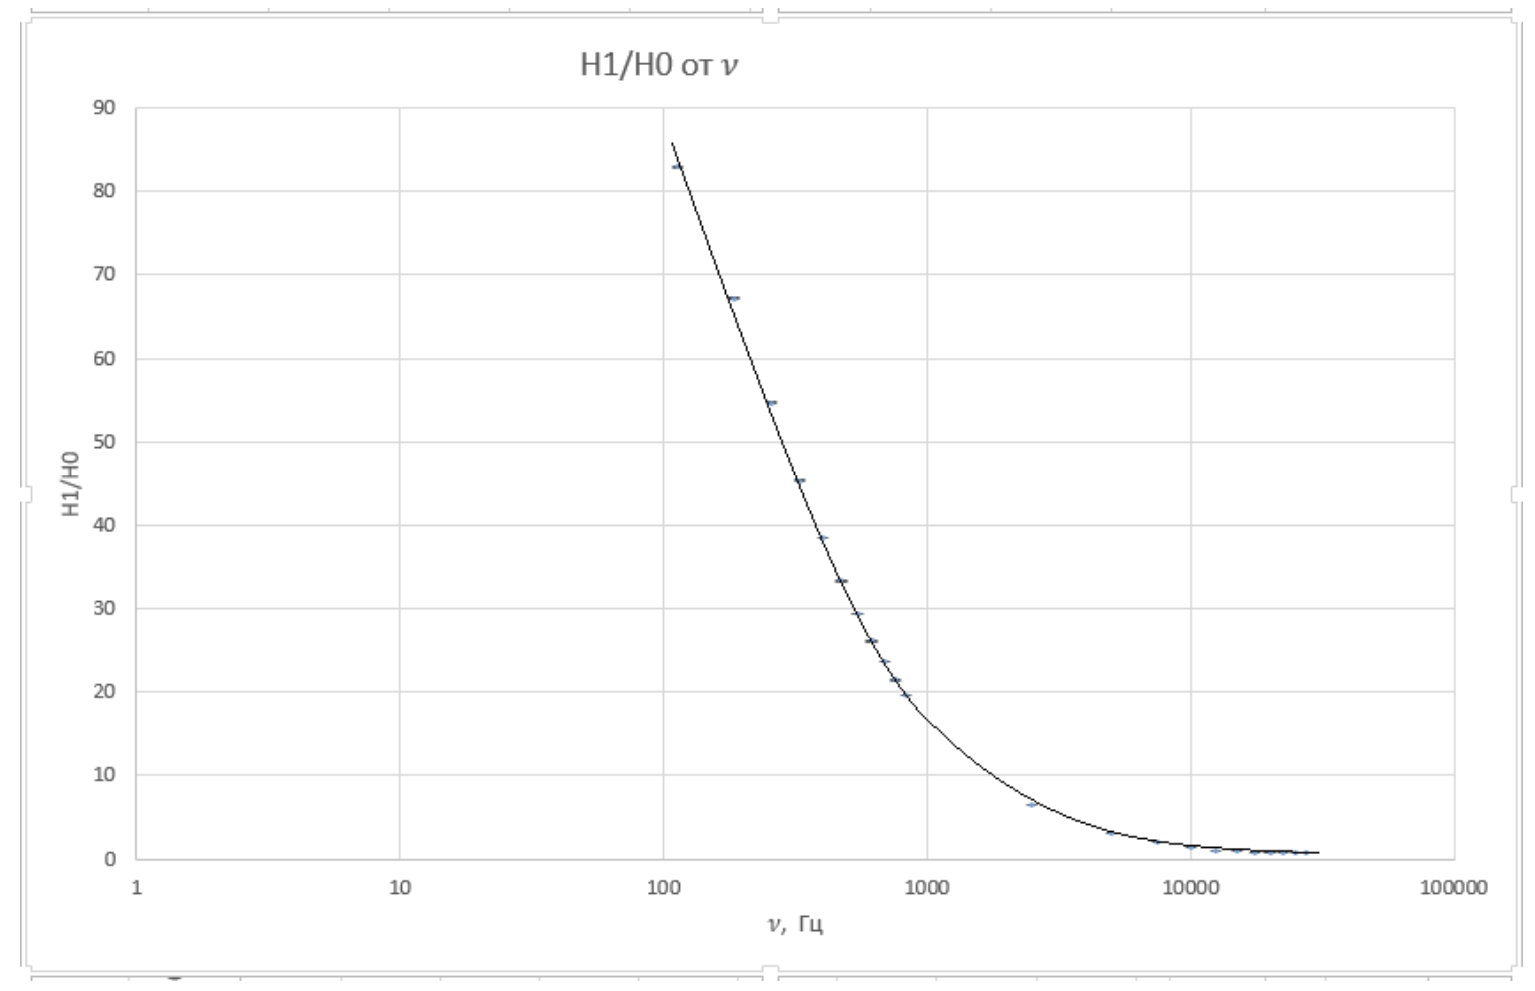
\includegraphics[scale=0.3]{PIC_7.png}
		\\\textbf{Рис. 7:} График зависимости $(|H_1|/|H_0|)(\nu)$
	\end{center}
	
	
	\newpage
	%Страница 9
	
	\begin{flushleft}
		\footnotesize{Скин-эффект в полом цилиндре} \hspace{\fill} \footnotesize{9}
		\\[-0.3cm]\noindent\rule{\textwidth}{0.3pt}
	\end{flushleft}
	
	
	
	\section{Выводы}
	
	В данной работе было исследовано магнитное поле в полом медном цилиндре. Линеаризованные графики зависимостей $1/\xi^2(\nu)$ и $\Delta \psi (\sqrt{\nu})$ показали справедливость теоретической модели скин-эффекта в цилиндре.
	
	По графику был определен коэффициент $\xi_0 = (1.6 \pm 0.03) \cdot 10^{-2} \left(\frac{\text{Ohm}}{\text{Hz}}\right)^2$
	
	По графикам также была найдена проводимость меди $\sigma$: 
	$$\sigma_{low} = (4.5 \pm 0.1) \cdot 10^7\,\frac{\text{S}}{\text{m}} \ \ \ \ \ \ \ \ \sigma_{high} = (7.0 \pm 1.2) \cdot 10^7\, \frac{S}{m}$$
	
	Эти значения близки к табличным: $(5 - 6) \cdot 10^7\, \frac{S}{m}$

	Была также показана зависимость $(|H_1|/|H_0|)(\nu)$.
	
\end{document}